% !TEX encoding = UTF-8
% !TEX TS-program = pdflatex
% !TEX root = ../tesi.tex

%**************************************************************
\chapter{Appendice A}
\section{Servizi di Angular 6}
 Un servizio in Angular 6 è una classe di tipo Singleton che implementa funzionalità condivise dai vari elementi di un’applicazione, siano essi componenti che altri servizi.
Ne esiste solo un istanza di uno servizio per tutta l'applicazione, in questo modo i dati condivisi dai diversi componenti sono gli stessi.
\\

L'implementazione di un servizio aviene utilizando il decorator @Injectable() di Angular. Questo decorator aggiunge alla classe dei metadati che permettono ad Angular di iniettare il servizio nei compoenti come una dipendenza. Viene utilizzato Dependency injection(DI) design pattern per iniettare le dipendenze dei servizi nei componenti. 
\begin{figure}[!h] 
	\centering 
	
\includegraphics[width=0.5\columnwidth]{DI} 
	\caption{Injector di Angular}
\end{figure}
\\

Dependency injection è utilizzato ovunque nel Framework Angular. In un'applicazione Angular un componente in media consuma molti servizi utilizzando DI, che li fornisce accesso a tutti i metodi e ai dati forniti dal servizio. 
\\ 

Quando un componente viene creato come prima cosa vengono controllate le sue dipendenze. Se il componente dipende da qualche servizio viene generato l'istanza Singleton di tale servizio(se non esiste già), in questo modo vengono soddisfatte tutte le dipendenze del componente prima della sua creazione. 
La Dependency injection è gestito dal oggetto injector di Angular, che ha il semplice compito di soddisfare le dipendenze. 
\begin{figure}[!ht] 
	\centering 
	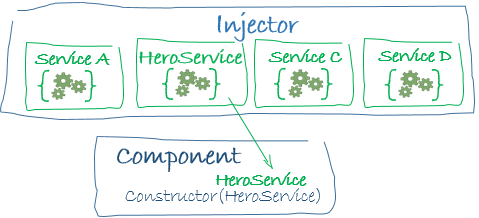
\includegraphics[width=0.7\columnwidth]{DI2} 
	\caption{DI in Angular}
\end{figure}
\section{RxJS in Angular 6}
RxJS (Reactive Extensions for JavaScript) è una libreria di reactive programming che permette di gestire le chiamate asincrone in maniera molto semplice.
\begin{figure}[!ht] 
	\centering 
	
\includegraphics[width=0.5\columnwidth]{rxjs} 
	\caption{Logo di Angular ed RxJS}
\end{figure}